\section{PhaistOS, le générateur d'ordonnanceurs d'E/S}
\label{intro}

\subsection{Quésaco}

``PhaistOS'' est le nom d'un Langage Dédié, ou Domain Specific Language (DSL) 
en anglais. Utilisé dans le domaine de l'ordonnancement des entrées/sorties (E/
S) d'un système d'exploitation (SE), il a pour but de faciliter la conception 
et la validation de politiques d'E/S écrite par un utilisateur. Il est le 
fruit issu du projet VeriAMOS (Verified Abstract Machines for Operating 
Systems) ayant pour but de s'attaquer au problème de vérification d'une classe 
de services de systèmes d'exploitation.

\subsection{La structure d'accueil}

Mon stage a donc porté sur le projet VeriAMOS, au sein de l'équipe Erods, 
accompagnée par les équipes Antique (INRIA Paris) et Whisper (Université de 
Sorbonne). Erods est une équipe de laboratoire qui étudie principalement la 
construction et la gestion de sytèmes cloud, en travaillant sur différentes 
facettes de ces derniers, comprenant la prise en charge d'environement 
d'execution distribué robuste et efficace. 

Erods fait donc parti du Laboratoire d'Informatique de Grenoble (LIG) avec 23 
autres équipes réparties sur 5 axes de recherches (voir Figure~\ref{fig:lig}). 
Ce laboratoire, reconnu internationalement, se base sur les sciences 
informatiques et cherche à approfondir ses concepts, allant jusqu'à la 
réalisation de maquettes innovantes qui anticipent les usages. Le laboratoire 
de recherche universitaire se situe sur le campus grenoblois de Saint Martin 
d'Hères (Université Grenoble Alpes (UGA)) et est composé de 500 chercheurs et 
enseignants chercheurs.

\begin{figure}[h!t] \centering
    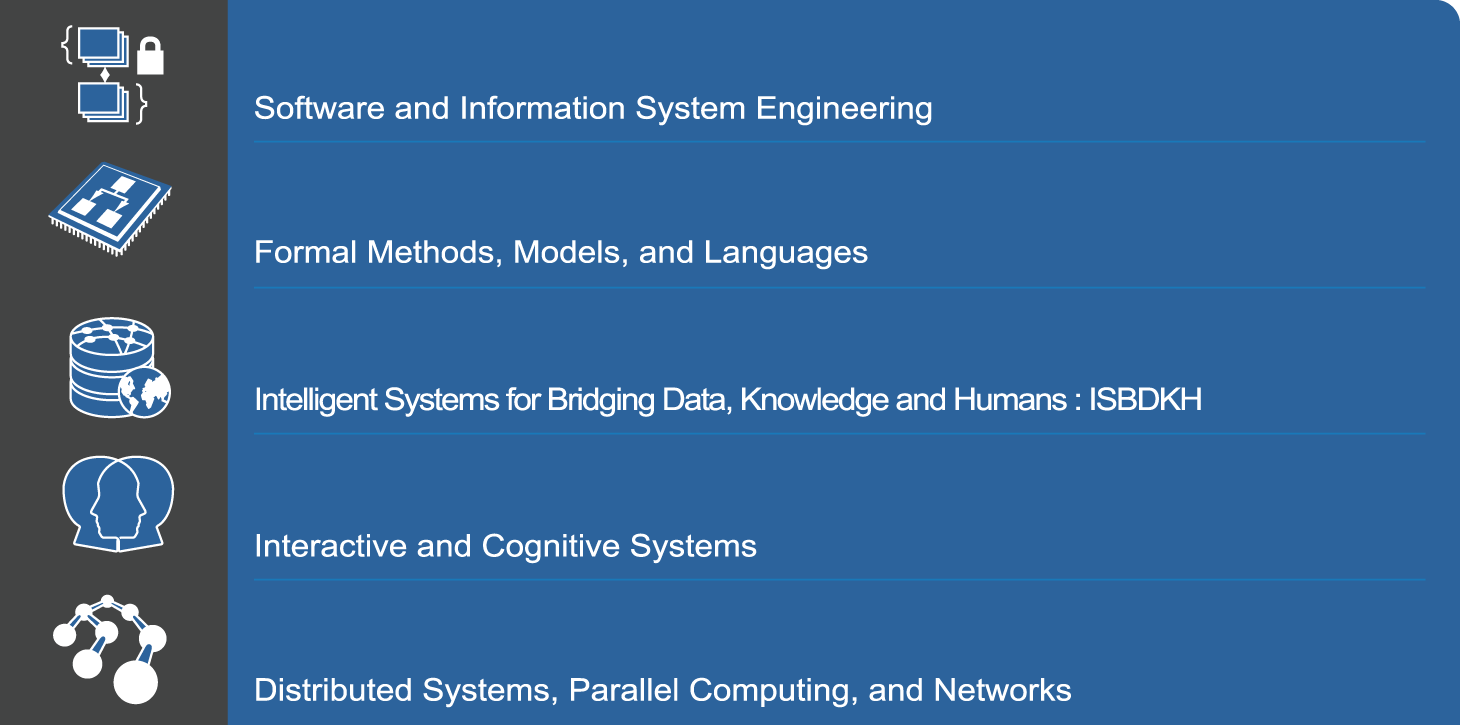
\includegraphics[width=12.5cm]{images/axeslig}
    \caption{Les différents axes de recherche du LIG.}
    \label{fig:lig}
\end{figure}

Mon employeur officiel reste donc l'université, c'est-à-dire l'UGA. Mon équipe 
et moi-même étions localisé sur le campus, plus précisément dans le bâtiment 
``IMAG'', au quatrième étage consacré à la recherche dans le domaine 
informatique (voir mon bureau sur la Figure~\ref{fig:imag}).

\begin{figure}[h!t] \centering
    \begin{tabular}{@{}c@{\hspace{5pt}}c@{}}
    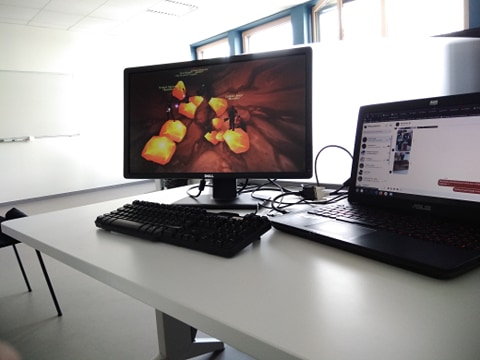
\includegraphics[width=0.49\textwidth]{images/desk} & 
\includegraphics[width=0.49\textwidth]{images/balcony}
    \end{tabular}
    \caption{Bureau de travail et balcon vu de la fenêtre.}
    \label{fig:imag}
\end{figure}

\subsection{Pourquoi PhaistOS ?}

Pour revenir sur le sujet de stage et le comprendre il faut tout d'abord 
expliquer pourquoi VeriAMOS à lieu d'être. En effet ce projet à pour but 
d'améliorer la vérification de systèmes d'exploitation, qui reste aujourd'hui 
compliqué pour deux raisons principales. Premièrement, les propriétés 
mathématiques des algorithmes sous-jacents sont généralement difficiles à 
exprimer, deuxièmement, la structure du code qui implémente ces algorithmes 
dans le SE est en général très complexe. 

Afin d'éviter de se retrouver dans cette situation d'un niveau de difficulté 
trop élevé pour effectuer une vérification efficace, VeriAMOS propose 
d'utiliser une technique d'abstraction basée sur un DSL (comme le fait 
Bossa~\cite{Barreto-Muller:asf2002}), ainsi qu'un analyseur statique, qui, à 
froid, pourra vérifier un ensemble de services fournis par le SE, comme par 
exemple celui de l'ordonnanceur des requêtes d'E/S.

Dans cette approche de développement système, le programme écrit avec le 
langage du DSL pourra être compilé pour générer un code source dans le langage 
du système et qui implémente le service visé (plus de détails Partie~\ref
{context}). En limitant ainsi la capacité d'expression du langage, le DSL 
contraint le programmeur et permet d'éviter une mauvaise utilisation des outils 
du langage cible, permettant ainsi d'améliorer la robustesse des services 
concernés du SE. Le développeur pourra donc se focaliser sur l'écriture de sa 
politique système de haut niveau et déléguera la génération de code au 
compilateur du DSL.

VeriAMOS offre une opportunité de formaliser et d'implémenter une nouvelle 
approche à la vérification de systèmes d'exploitation, sur différents services. 
Ici nous nous focaliserons sur celui de l'ordonnanceur d'E/S du système, mais 
nous pensons que cette approche reste générale et pourrait s'appliquer sur tout 
types d'ordonnanceurs, de systèmes de fichier, etc.

\subsection{Mon rôle dans ce projet}

Pour résumer grossièrement, PhaistOS se décompose donc en deux parties 
principales : le compilateur et l'analyseur, ma mission portant uniquement sur 
le compilateur, ou autrement dit, le générateur de code C. 

En effet, le but de ma mission était de faire évoluer le compilateur actuel 
pour qu'il puisse produire un code qui se rapproche de celui d'un module Linux.
Un module Linux étant une extension du noyau du système qui peut être branchée
et débranchée à volonté, à chaud, c'est-à-dire pendant que le système est 
chargé en mémoire RAM et s'éxecute. À cet objectif se rajoute celui de tests 
d'analyses comparatives ayant pour but de montrer que l'utilisation d'un DSL 
n'a que très peu d'impact sur les performances finales du code généré. Bien 
évidemment, d'autres tâches me seront assignées, comme celle de la 
documentation, ou de la paricipation à la rédaction du papier scientifique 
portant à décrire le fonctionnement de PhaistOS (plus de détails sur ma 
contribution au projet dans la Partie~\ref{contrib}).

\subsection{Pré-requis}

Avant de commencer ma mission, il a fallut que je me familiarise avec mon 
environement de travail, surtout avec les outils que j'allais utiliser. Pour 
comprendre et bien aborder ce qui allait suivre, j'ai du lire des extraits de 
documentation, des pages de wikis, et même des fois des forums.

La première étape a été de comprendre comment les ordonnanceurs d'E/S 
fonctionnaient sous Linux. À savoir, que chaque ordonnanceur est considéré 
comme un module (intégré de base dans le SE ou non), et que l'ordonnanceur 
actif est contenu dans un fichier particulier du système (changer le contenu du 
fichier change l'ordonnanceur actif).

Il a fallut ensuite que je me familiarise avec l'environement de travail 
virtuel qui m'était proposé, c'est-à-dire le ``déjà existant'' du projet, 
comprenant la documentation, les exemples, le moyen employé pour implémenter 
PhaistOS dans le système et pour finir le code source de PhaistOS des 
différents dépôts de système de versions Git hébergés sur la plateforme \href
{https://gitlab.inria.fr/}{Gitlab}.

Plus tard, j'ai du utiliser un réseau de serveurs externes appelé Grid'5000 
pour effectuer des tests sur des machines plus performantes que ma machine 
personnelle. Pour cela j'ai du respecter une charte d'utilisation et apprendre 
les commandes propres à l'utilisation de la plateforme. À ce niveau là du 
stage, une connaissance fondamentale des systèmes d'exploitation était 
nécessaire pour chaque installation sur les machines distantes.

La dernière étape a été de ... 